\chapter{Details}\label{chap:details}
\section{Kalman Filter}
Part of the challenge of implementing a Kalman filter for this lab was to appropriately tune the $\sigma_x$ matrix.  In its original form, we allowed an extremely large value for the $x$ and $y$ acceleration parameters---on the order of 100 or so.  The result was a very loose guess that produced exaggerated acceleration and velocity vectors.  Although the position vector was not too far off, the effect of a wildly inaccurate velocity vector was that our ``hunter'' tank overcompensated for the velocity on all counts.  Next, we tried narrowing the values a bit, hoping that by reducing the parameters we would tighten the difference between observed values and filtered values.  In this we were partially successful---by using $0.001$ for the position vector, $0.01$ for the velocity vector, and $0.1$ for the acceleration vector, our Kalman filter seemed to train fairly well on the varying data.  With a little room for error, and this tighter range, our hunter was able to shoot down all of the clay pigeons except for our ``wild'' pigeon, the one that moved in a non-gaussian manner.

One interesting observation was that it was actually ok to have a slightly inaccurate filtered position vector as long as the velocity was also only slightly inaccurate.  Smoothing out the position vector by increasing its variance did not improve our odds.  Therefore, it was tuning the velocity vector's accuracy that most helped us to achieve reasonable hunting results.

In all of the screenshots below the significance of coloration will follow this format:
\begin{itemize}
    \item red lines - observed locations connected in chronological order
    \item green lines - filtered locations connected in chronological order
    \item yellow lines - normals representing levels of uncertainty around our ``best-guess'' of the location of the other tank
\end{itemize}
\begin{figure}
   \begin{center}
   	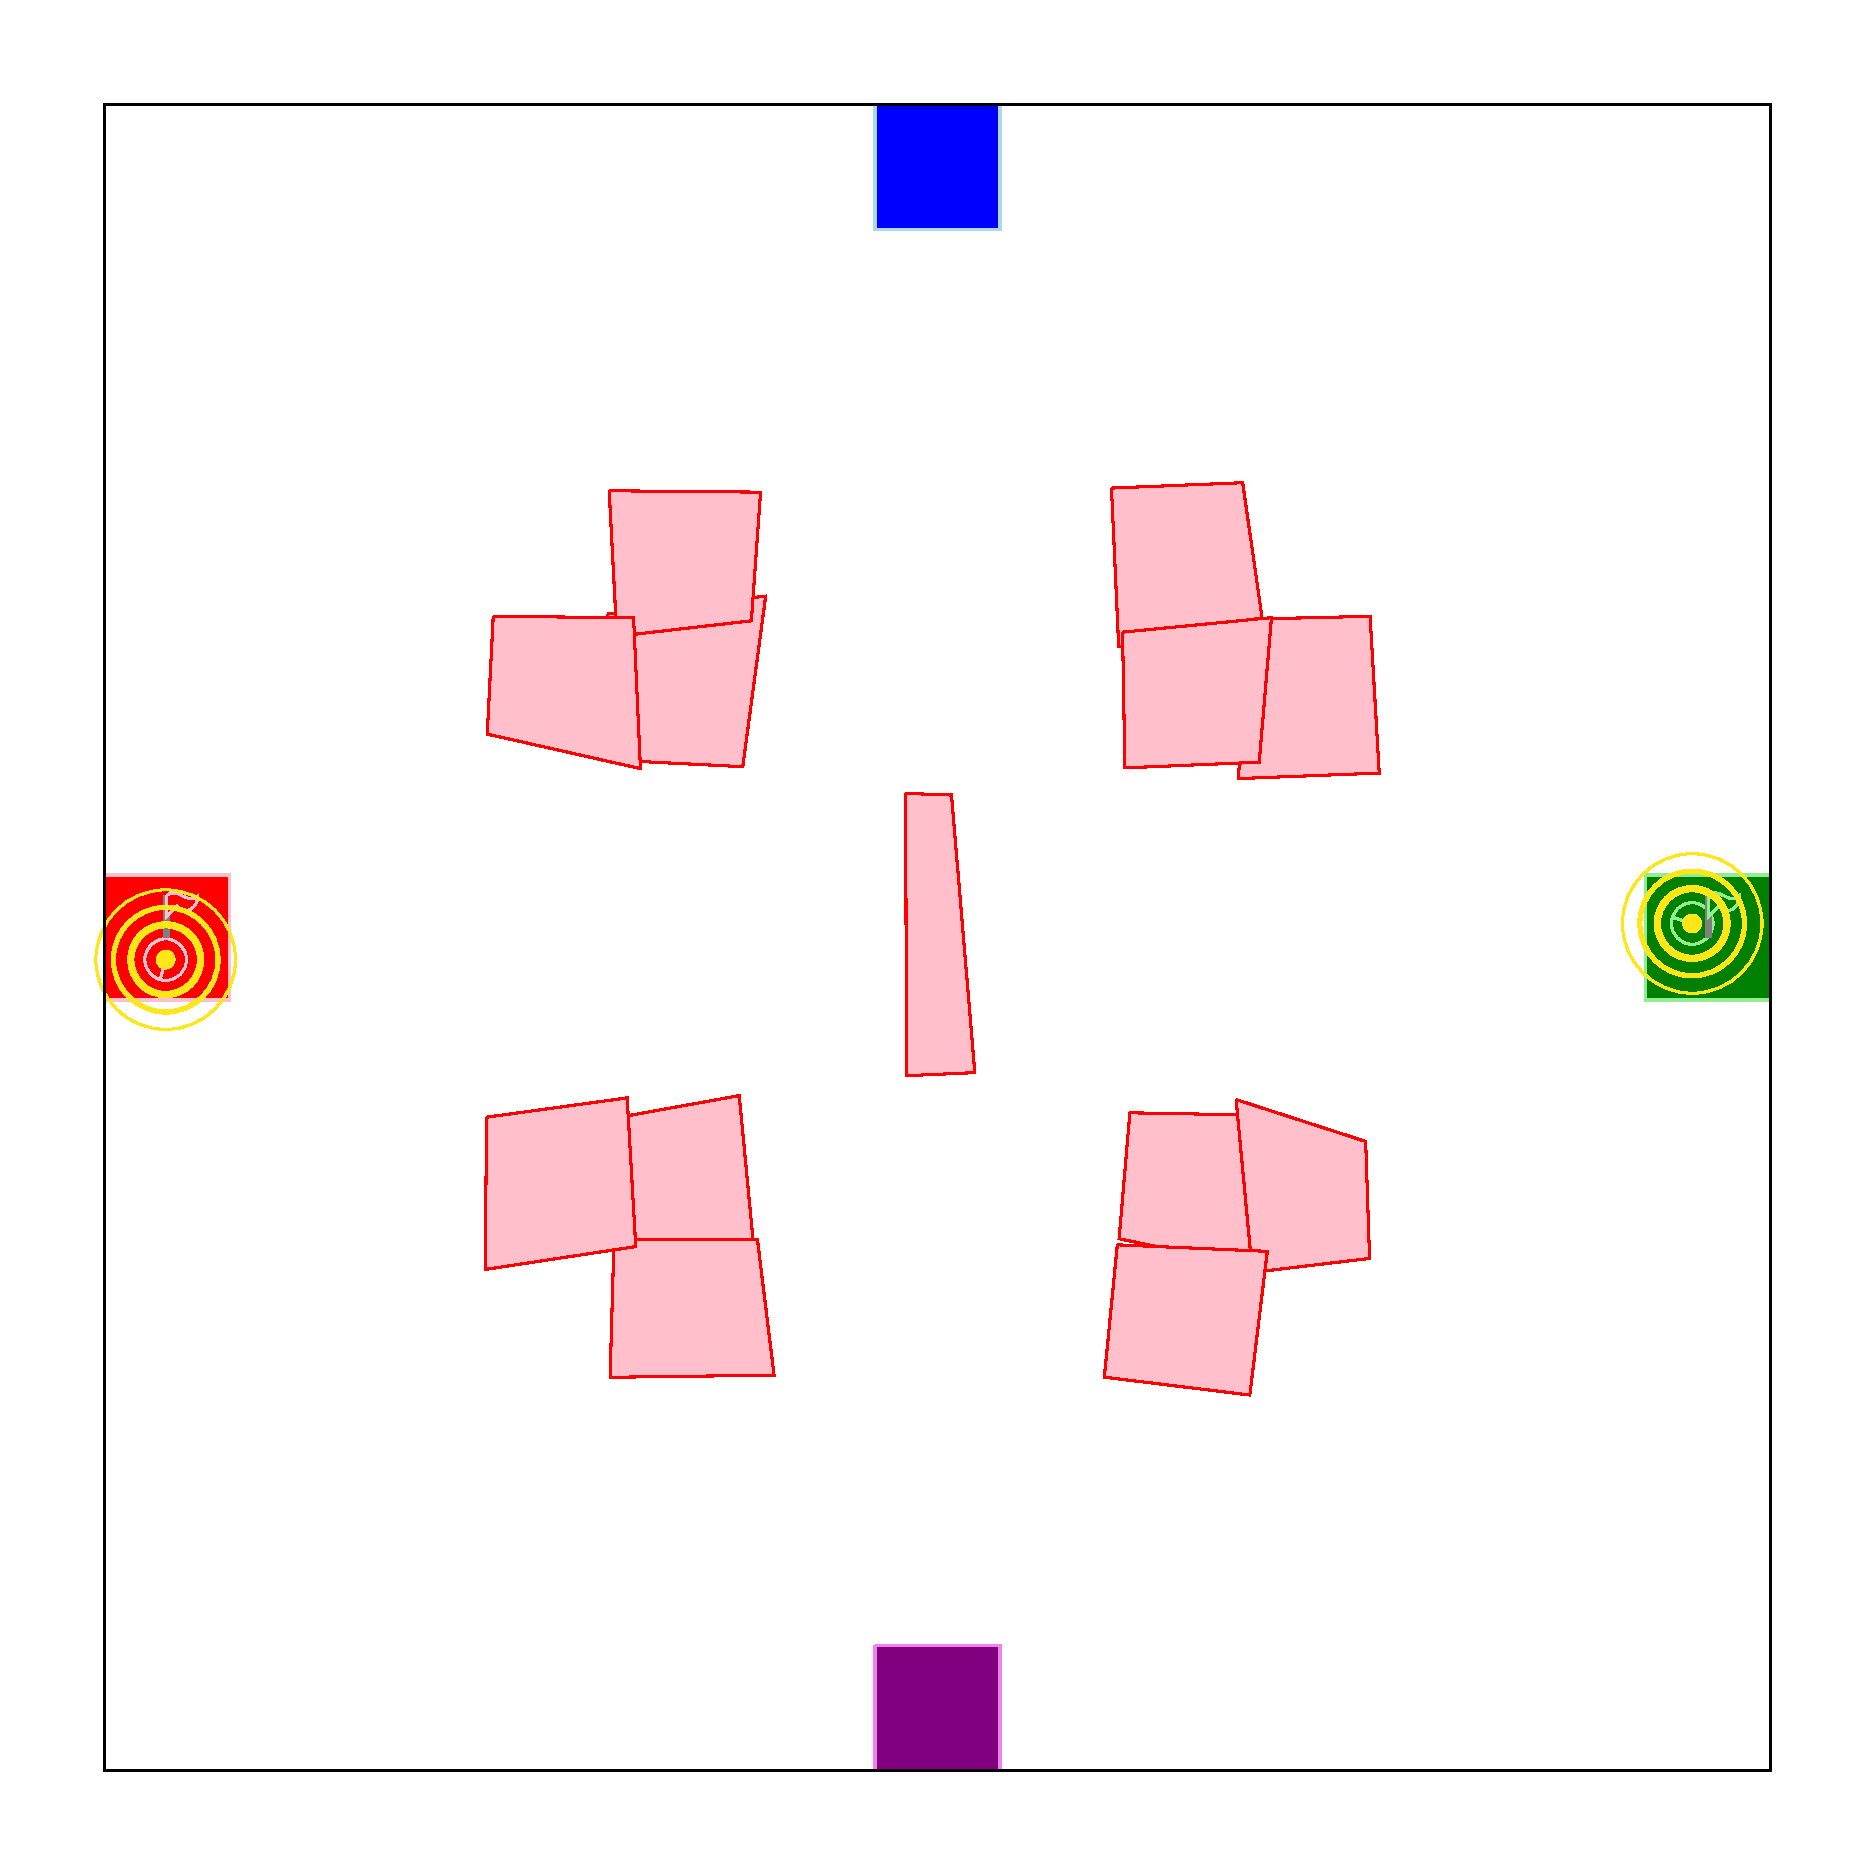
\includegraphics[width=\textwidth]{wackyworld.png}
   \end{center}
   \caption{A view of the world as seen with ``noisy'' sensors}
  \end{figure}
\section{Clay Pigeons}
As part of this lab we designed some simple ``Clay Pigeon'' agents to shoot at.  They displayed various characteristics and served as a way to judge how effective our Kalman filter was at judging the position, velocity and acceleration of tanks on the field.
\subsection{Conforming Pigeons}
The confoming pigeons were pretty boring as far as implementation goes. Jon created the following conforming pigeons:
\begin{itemize}
    \item Sitting duck - sat still waiting to be shot
    \item Constant Velocity - drove in a straight line at a constant velocity
    \item Constant Acceleration - Accelerated in a constant way
    \item Gaussian Acceleration - Accelerated in x and y according to a gaussian distribution.
\end{itemize}
The only thing worth nothing about these implementations is that they were progressively harder for our Kalman agent to shoot.  Also we used two types of constant acceleration.  One type kept a constant velocity and angular velocity and essentially drove in circles always accelerating towards the center.  The other implementation actually changed its forward velocity and angular velocity in a consistent way.  Both were somewhat difficult for our agent to hit.
\begin{figure}
   \begin{center}
   	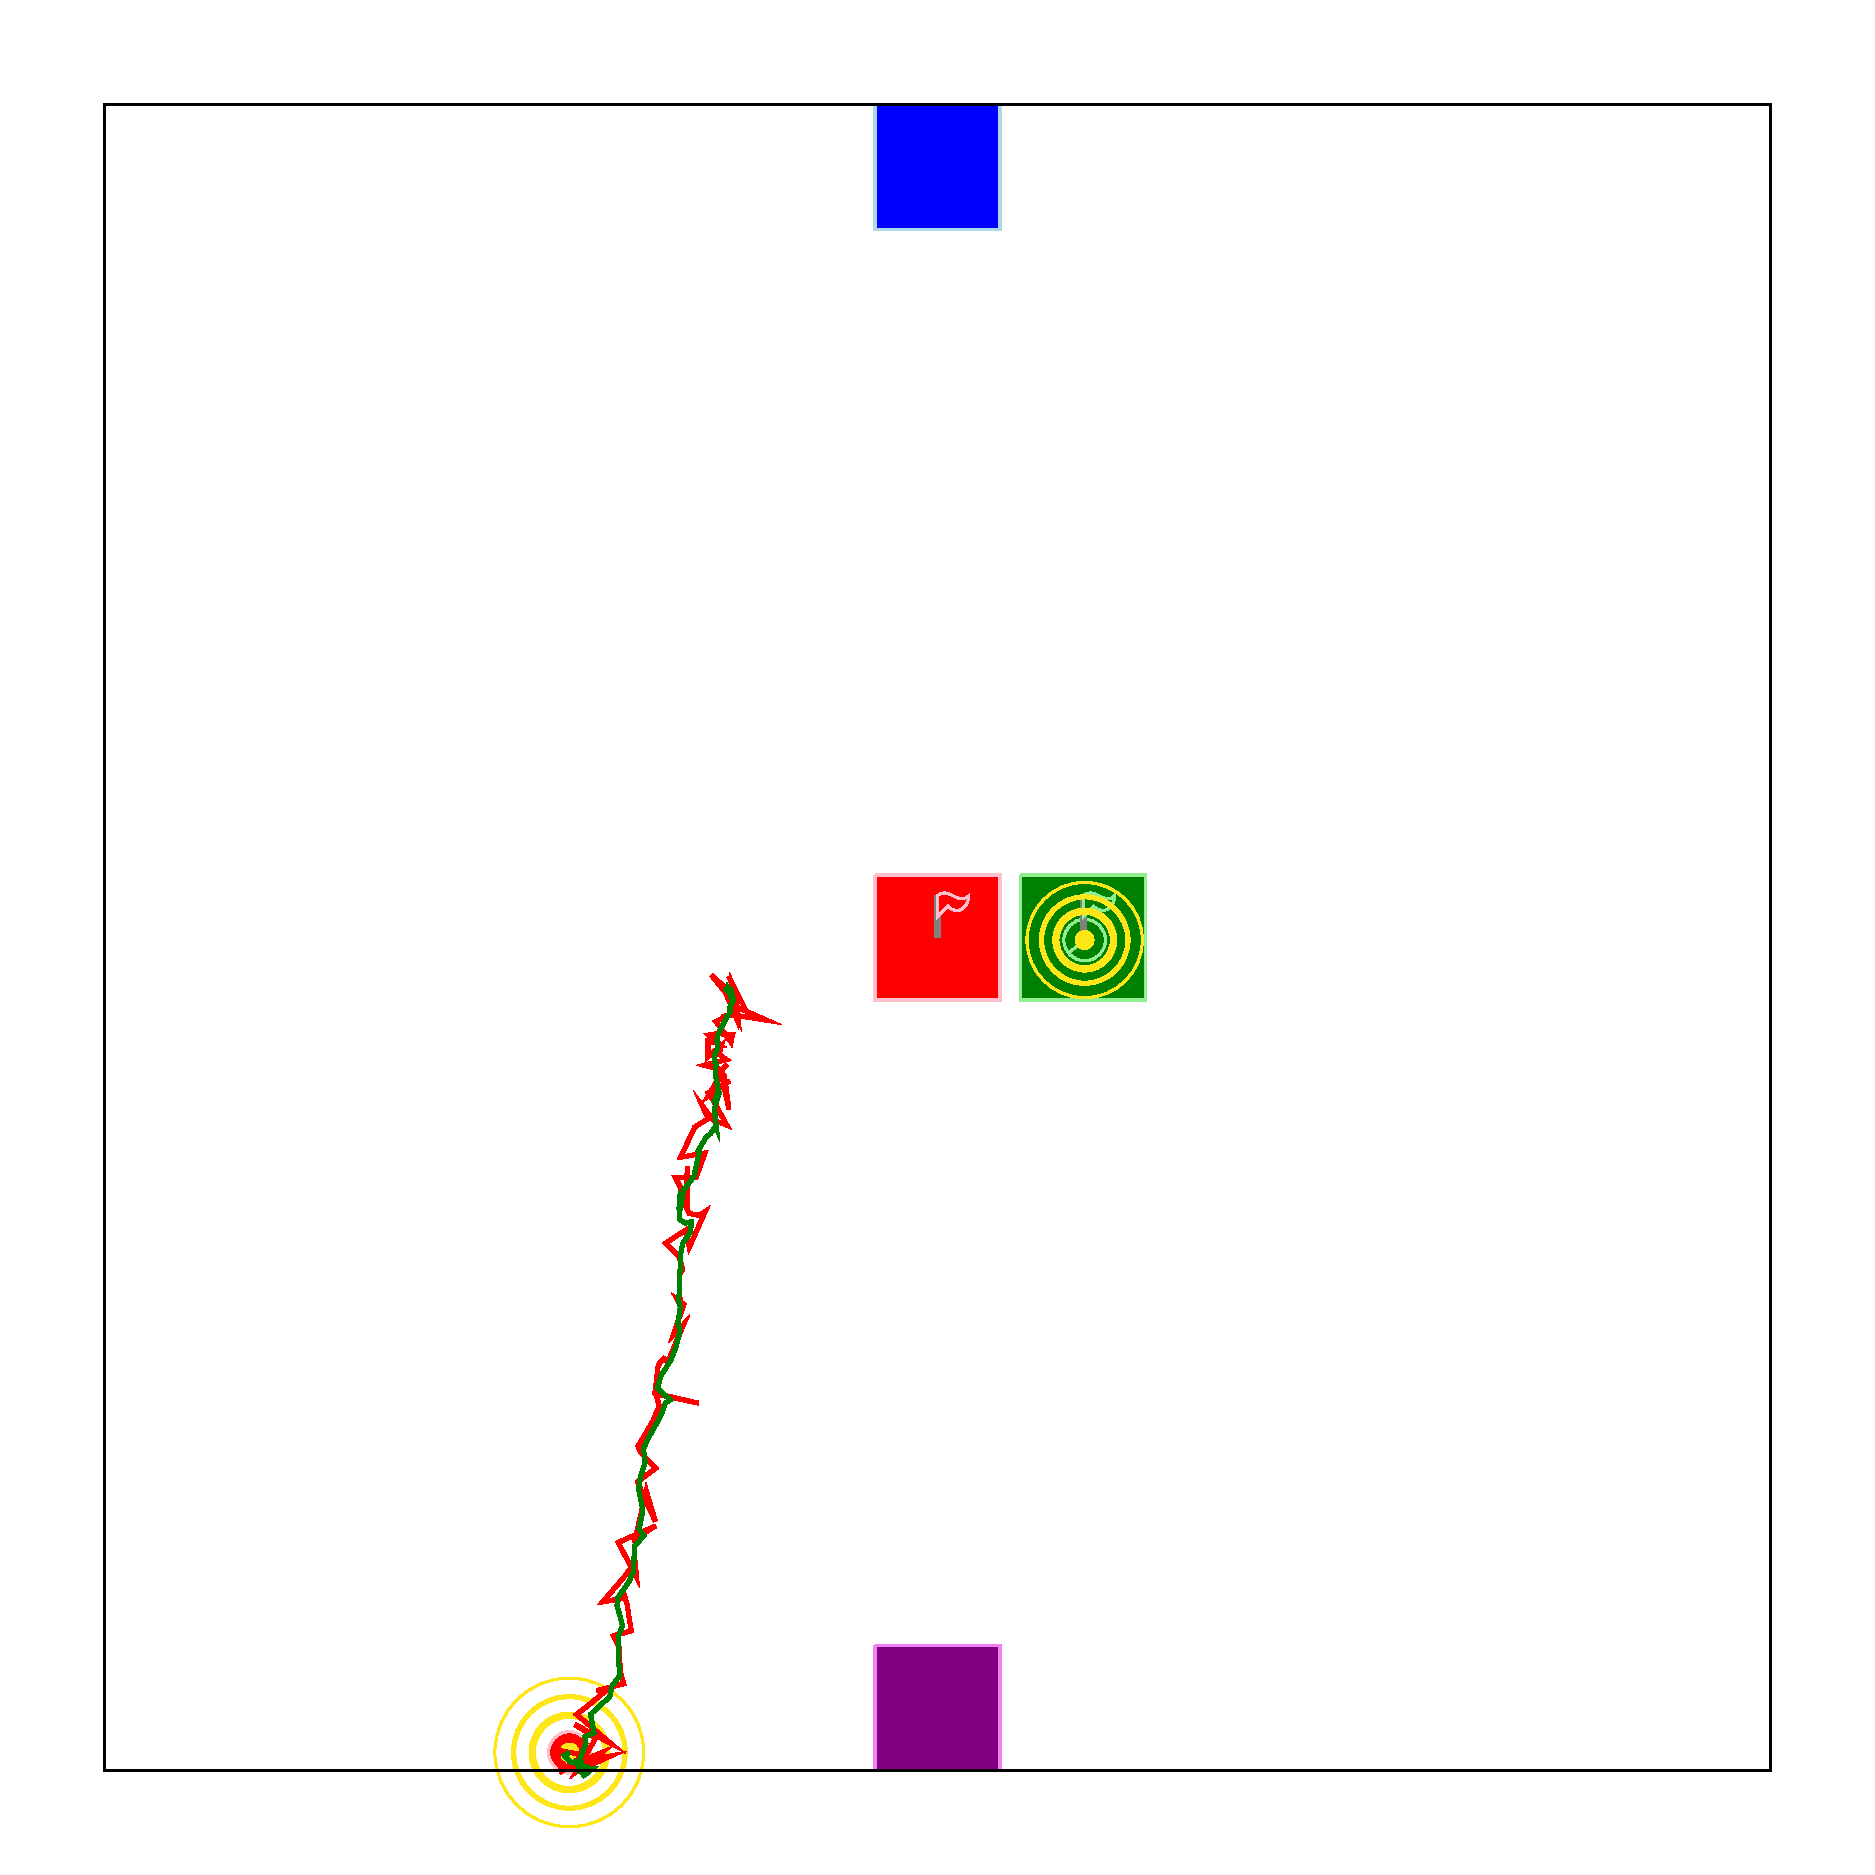
\includegraphics[width=\textwidth]{kalman-path-cv1.png}
   \end{center}
   \caption{Our Constant Velocity Clay Pigeon}
  \end{figure}
\begin{figure}
   \begin{center}
   	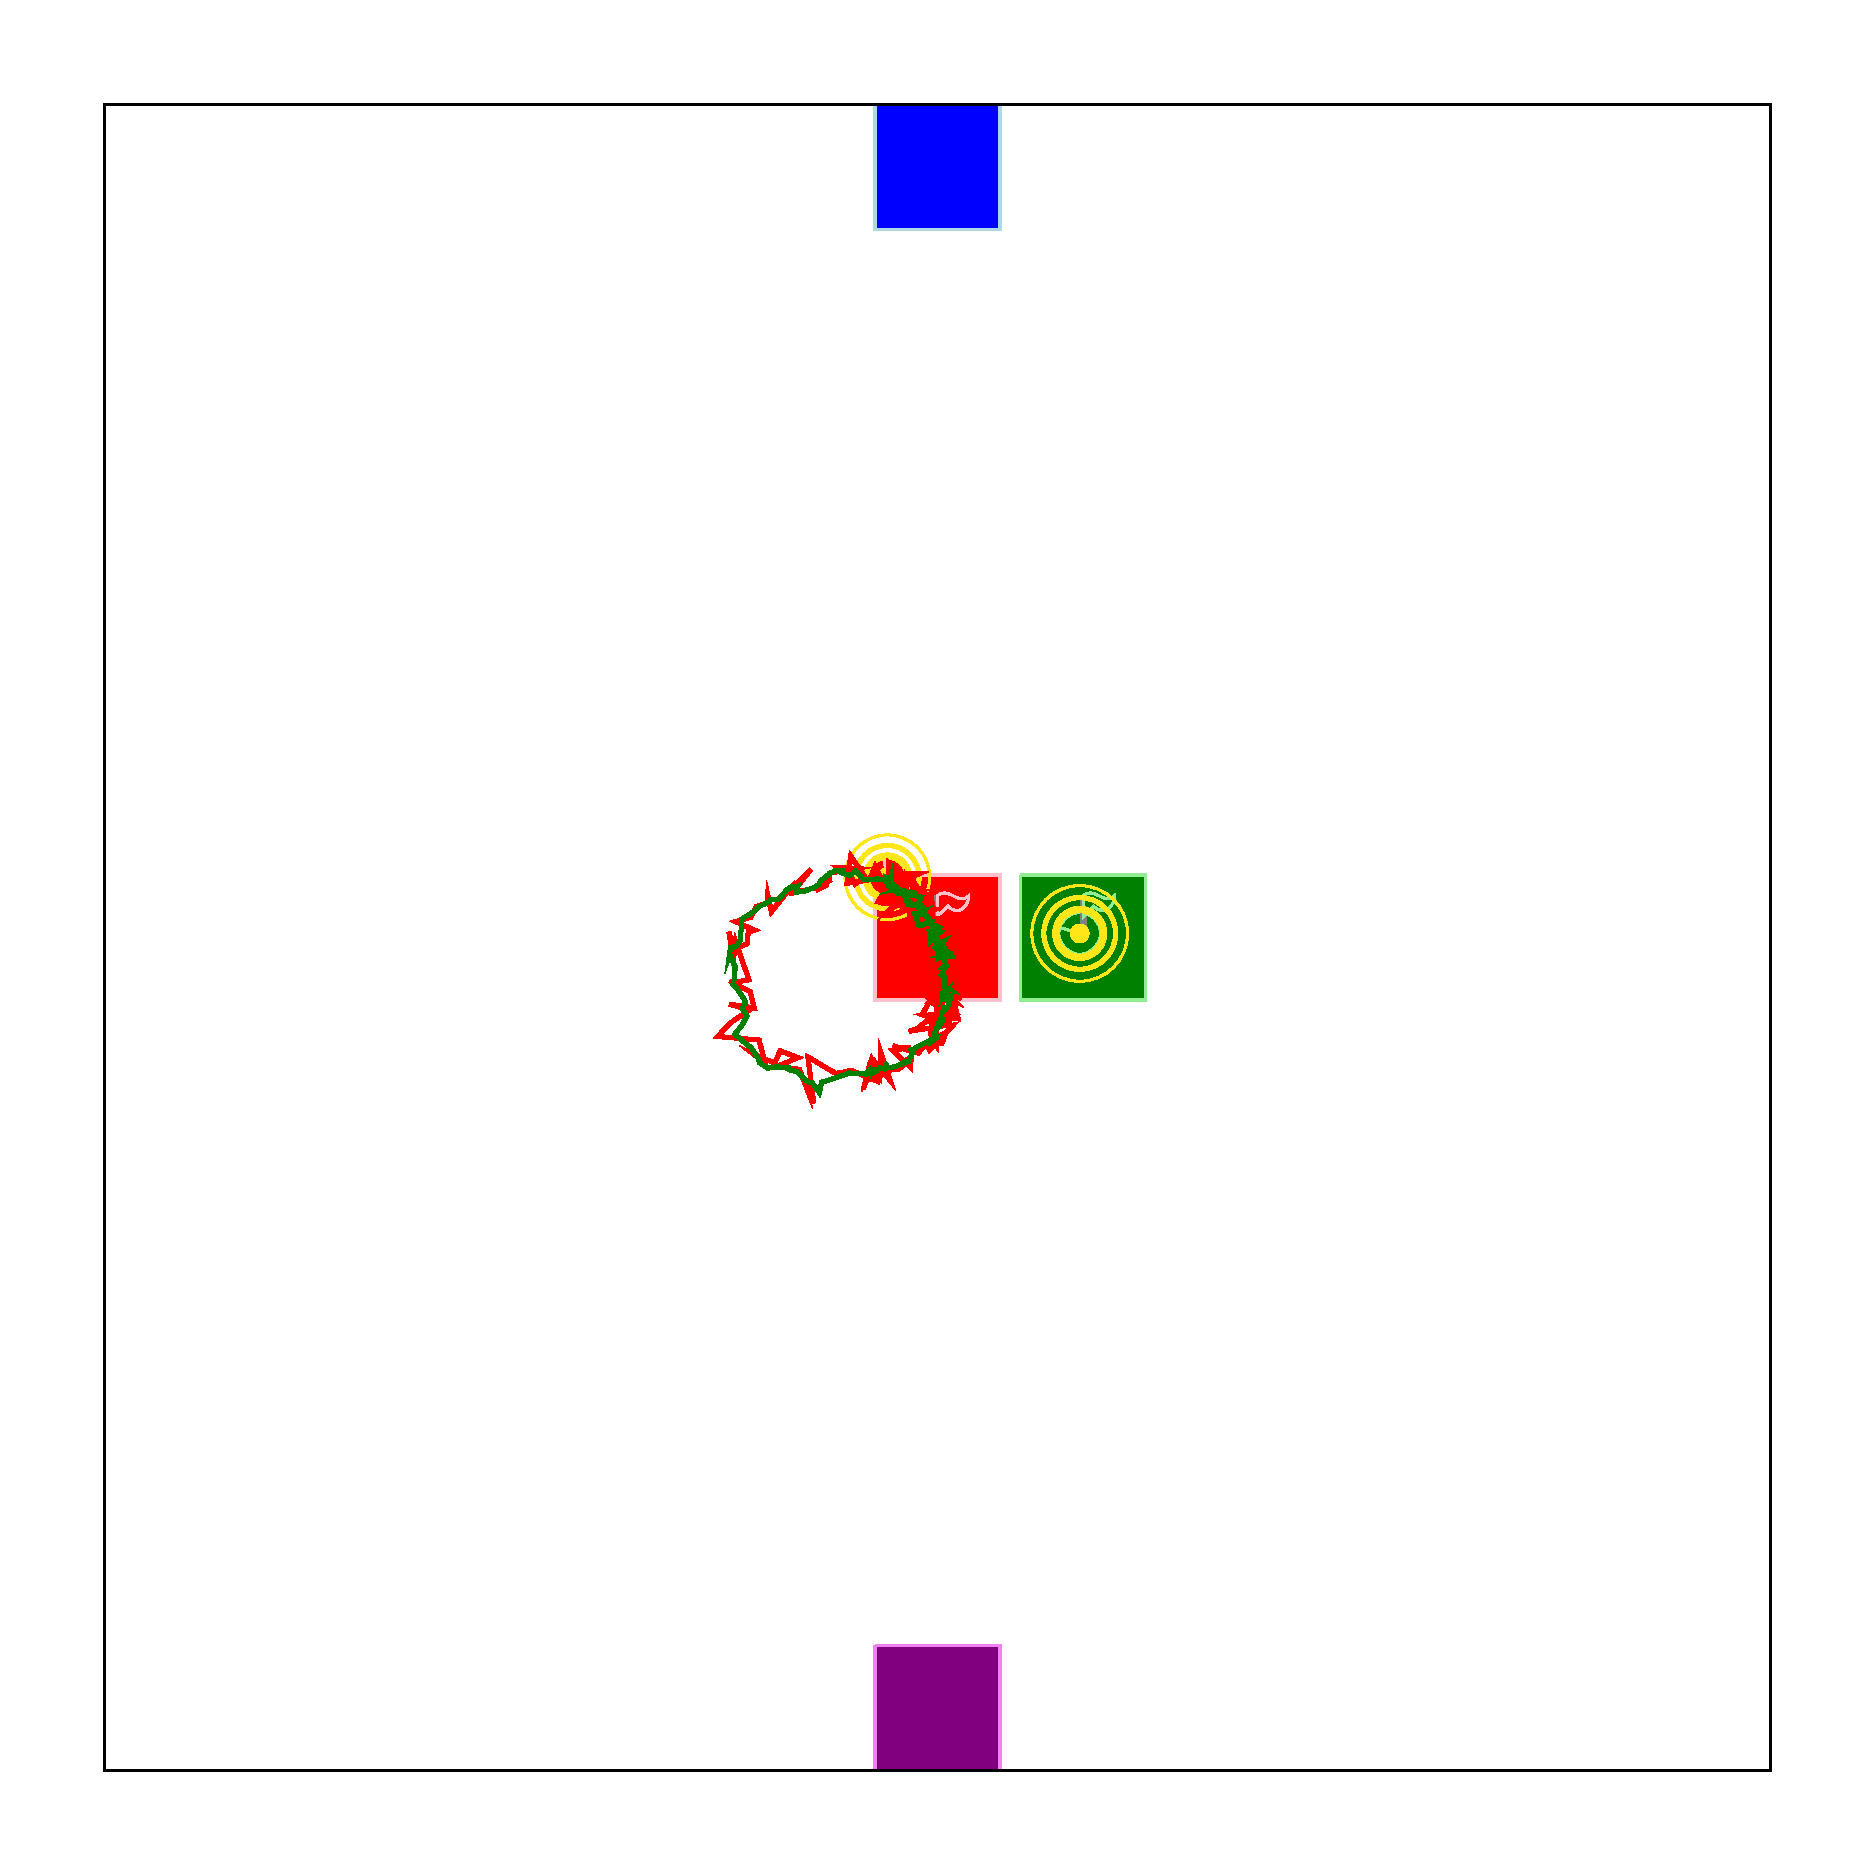
\includegraphics[width=\textwidth]{kalman-path-ca1.png}
   \end{center}
   \caption{Our Constant Acceleration Clay Pigeon}
  \end{figure}
\begin{figure}
   \begin{center}
   	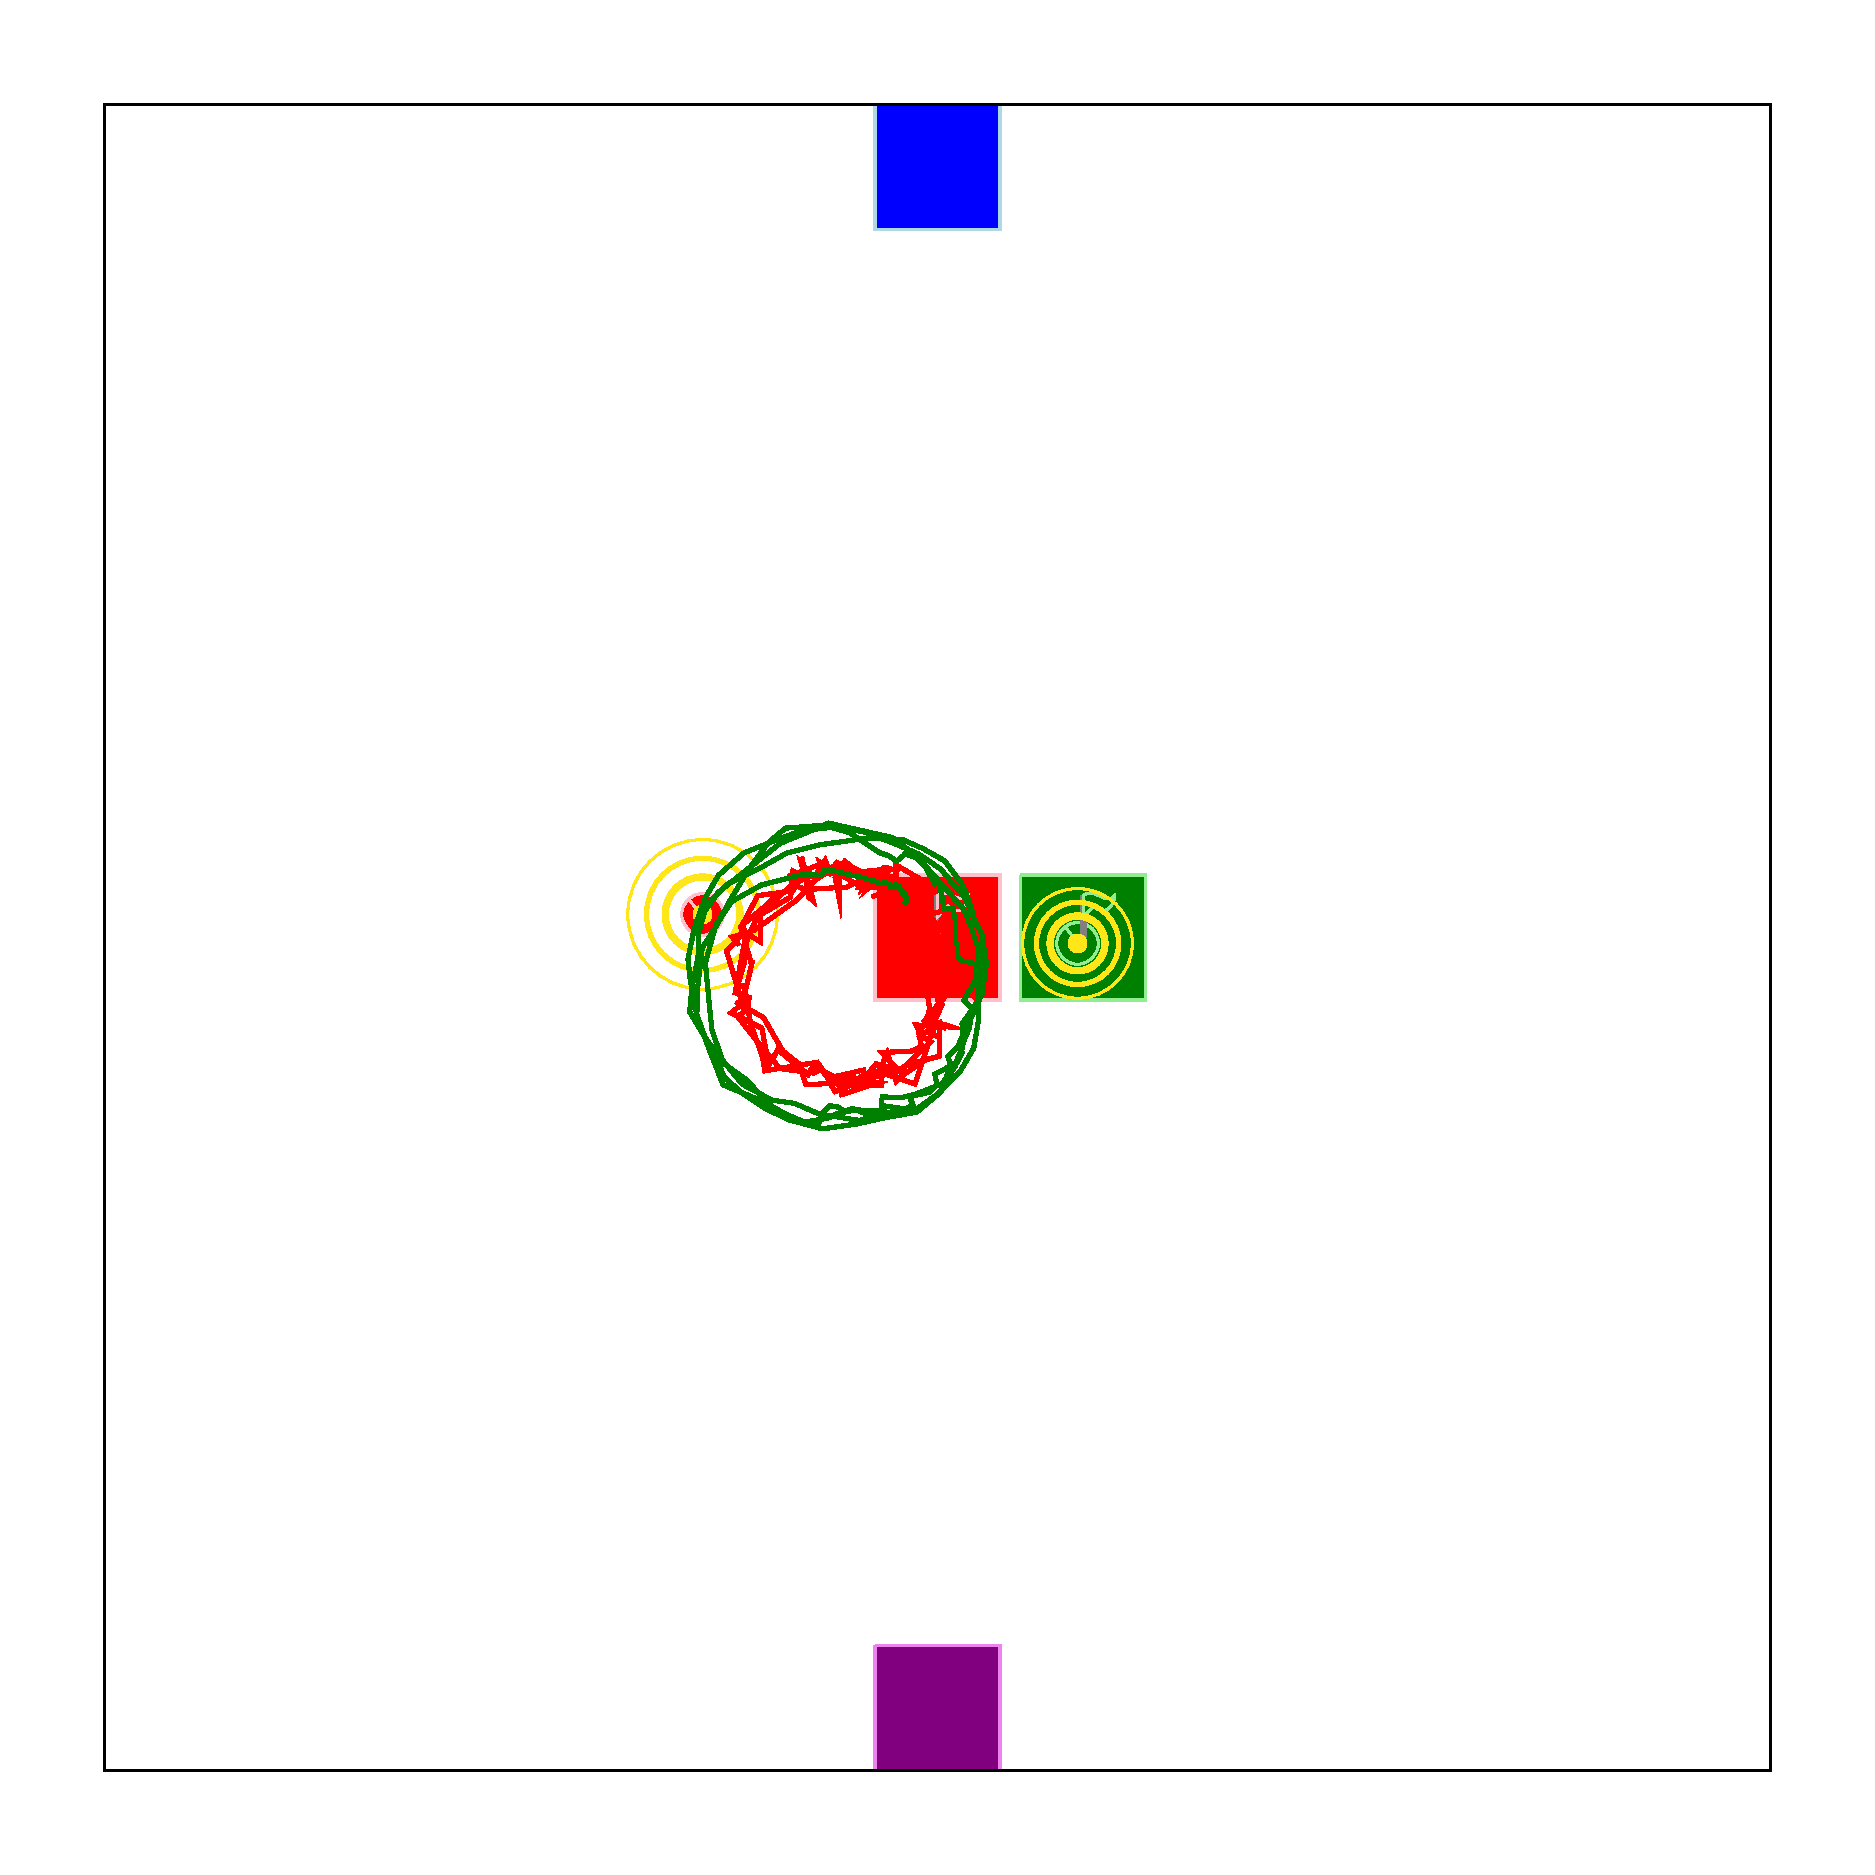
\includegraphics[width=\textwidth]{kalman-path-ca2.png}
   \end{center}
   \caption{Our Constant Acceleration Clay Pigeon}
  \end{figure}
\subsection{Non-Conforming Pigeon}
We designed the non-conforming pigeon to exploit the deficiencies in the Kalman filter.  We did this by recognizing that by changing the behavior of the robot over relatively short periods of time (2.5 seconds or less) we could deceive the filter since it relies on good readings over a reasonable length of time.
\par
The further away the pigeon is from the targeting tank, the more effective the technique because the time in which the tank needs to calculate the position of the pigeon to both predict and make the shot are less than the amount of time it takes for the pigeon to change its speed or angular velocity.
\par
We designed the pigeon to behave as follows.  We decided to use two separate timers, one for the speed and the other for the angular velocity.  Each timer was randomly set between 1 to 25 time steps, where each time step was defined as a tenth of a second.
\par
Initially the time steps were set to between 1 to 100 for a maximum of 10 seconds, but we realized pretty quickly that this was far too long for it to deceive the filter.
\par
At each iteration we decremented both timers and reset them when they hit zero.  When the timers are reset we calculate and set the new speed and/or angular velocity.
\par
In practice this technique proved to be effective since over a period of fifteen minutes the pigeon was hit only one time.  We had some other ideas that we had thought about exploring if the original implementation did not perform as well as we would have liked, however the pigeon did not disappoint, thus no other algorithms were devised.
\par
In planning for the tournament, we recognize that one easy way to negate the performance of the non-conforming pigeon is to move within a much closer shooting distance.  By doing this the amount of time between change in behavior and the filters ability to accurately predict the range will be long enough for the tank to make accurate and deadly shots.
\begin{figure}
   \begin{center}
   	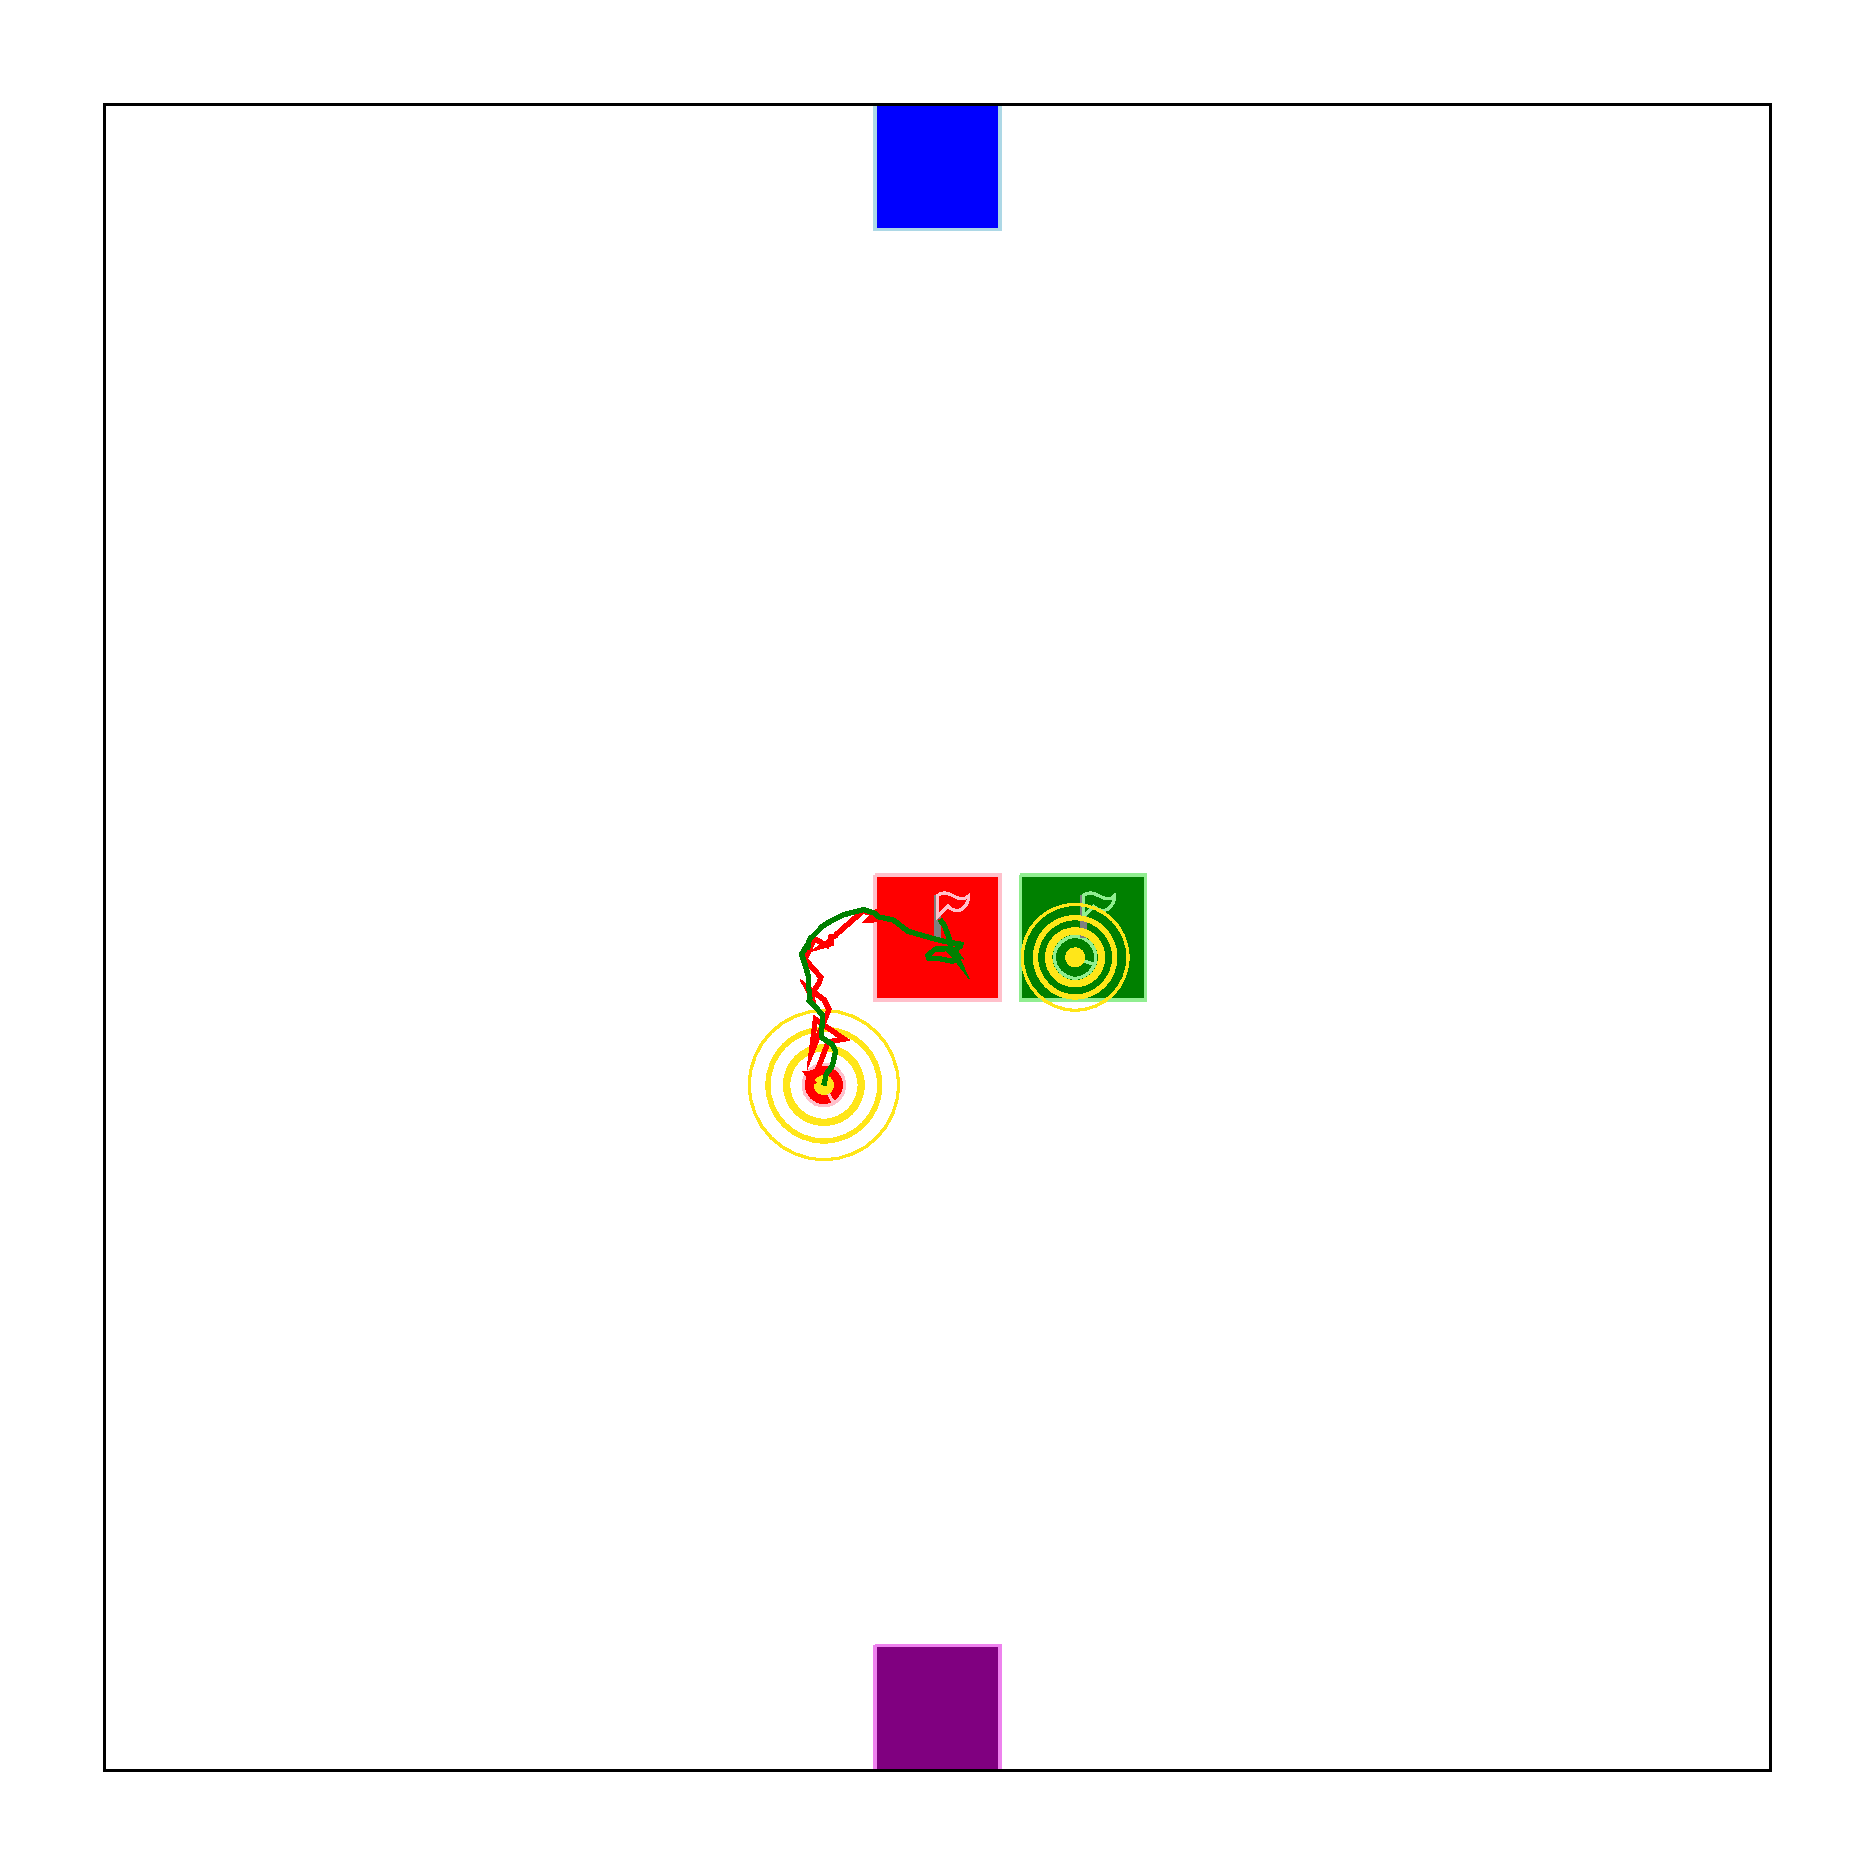
\includegraphics[width=\textwidth]{kalman-path-wild1.png}
   \end{center}
   \caption{Our Wild Clay Pigeon}
  \end{figure}
\begin{figure}
   \begin{center}
   	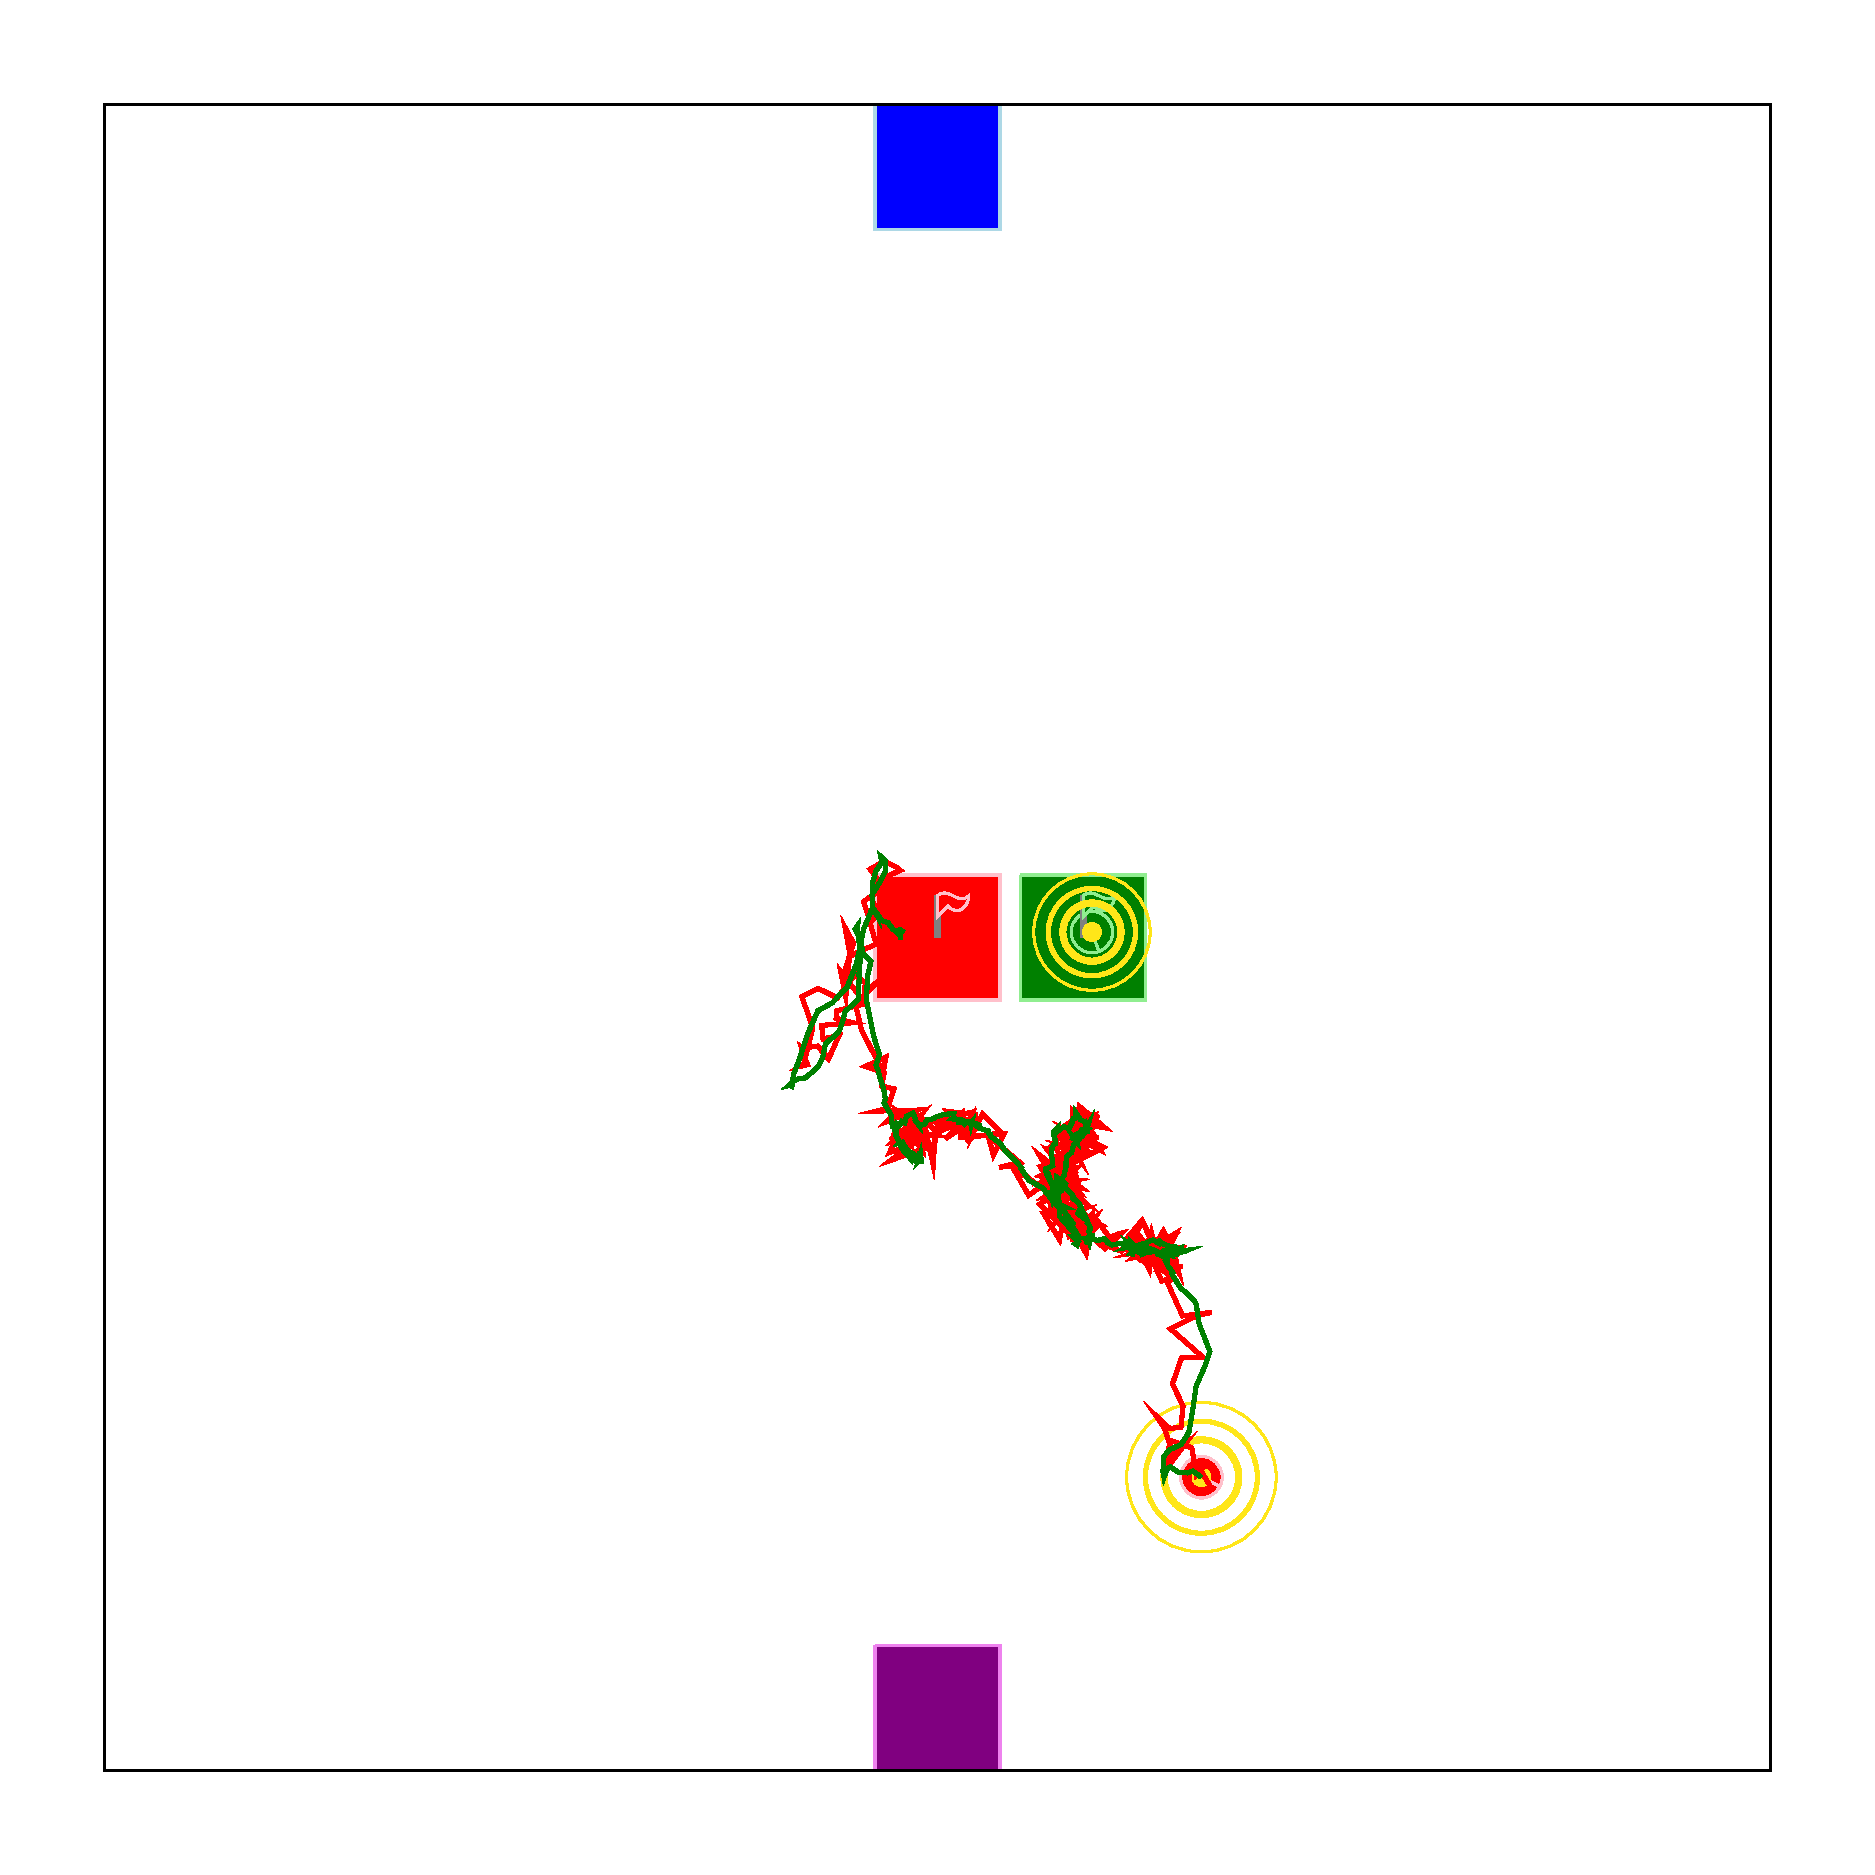
\includegraphics[width=\textwidth]{kalman-path-wild2.png}
   \end{center}
   \caption{Our Constant Velocity Clay Pigeon}
  \end{figure}
\section{Tests with Another Group}
\subsection{Our Tests}
Our tests were executd in a simple bzflag world with the red and green base near the center and the map was devoid of obstacles.  This helped to keep us focused on the goals of this lab.  In the last round of tests our agent was very accurate in killing the conforming clag pigeons.  It took between three and five shots to kill each conforming clay pigeon.  This was observed when killing both our clay pigeons and the other team's clay pigeons.
\par
The wild pigeons proved to be very wild.  Because every aspect of the wild pigeons behavior changed we were unable to find a good way to target it.  We tried various techniques.  Mostly we tried changing our Kalman filter to believe more strongly in the current observations than in its previously filtered values.  This change helped and ultimately the wild pigeon wandered close enough and while making a turn the kalman agent destroyed it.  A simliar experience with the other team's wild pigeon took place.  When the wild pigeons make truly random changes to velocity and angle we found no good way to predict their location.  Our inability to predict translated into a poor chance of shooting the wild pigeons.
\subsection{The Other Team}
We ran our battery of tests and observed the tests of two other groups:
Group 1
\begin{itemize}
    \item{Dave Brinton}
    \item{Tracen Peterson}
\end{itemize}

Group 2
\begin{itemize}
	\item{Matt Chou}
	\item{David Wilcox}
	\item{Kendell Clement}
\end{itemize}
\par
Watching the other teams agents, and passing off against their pigeons was interesting.  All three teams seemed to be almost equally efficient in their ability to kill the clay pigeons, but the defects in each agent were different.  Dave Brinton's group seemed to have some problems with turning to the right angle and so they missed about equally to the right or left of the pigeon.  Our agent seemed to have difficulty with agents moving quickly.  It would try to shoot too far in front of the pigeon and would always end up missing in front of the pigeon.  This is probably because of some ``fudge factors'' that we built into the agent to give it a sense that turning was not instantaneous.  This deficiency will have be addressed for the final lab.  Matt Chou's group seemed to have the opposite problem as we did and they consistently shot too far behind the clay pigeons.  They seemed to think that the PD controller was keeping them behind the desired angle as it slowed before reaching its optimal angle.
\par
The pigeons from each group were very similiar.  In fact the behaviour of all the conforming pigeons was nearly identical and only seemed different between the implementations of the gaussian acceleration pigeon.  But even with the guassian acceleration pigeon the results were similar as to how quickly the pigeons were shot.
\par
The wild pigeons were suprisingly similiar although each seemed to favor randomness in a different way.  None of the teams seemed to have a good way to change their Kalman filters to adapt to the wild pigeons.
\par
The code from the other teams looked good.  Dave Brinton's group had code that looked a lot like ours because the syntax was the same.  We noticed their code was full of printf statements used to debug strange behavior in their Kalman filter.  Matt Chou's group had very organized code which was a bit more verbose because it was written in Java.  All three teams used matrix libraries to solve the three central equations of the Kalman filter.